\documentclass[journal,12pt,twocolumn]{IEEEtran}

\usepackage{setspace}
\usepackage{gensymb}
\singlespacing
\usepackage[cmex10]{amsmath}

\usepackage{amsthm}

\usepackage{mathrsfs}
\usepackage{txfonts}
\usepackage{stfloats}
\usepackage{bm}
\usepackage{cite}
\usepackage{cases}
\usepackage{subfig}
\DeclareMathAlphabet{\mathpzc}{OT1}{pzc}{m}{it}
\usepackage{longtable}
\usepackage{multirow}
\usepackage{enumitem}
\usepackage{mathtools}
\usepackage{steinmetz}
\usepackage{tikz}
\usepackage{circuitikz}
\usepackage{verbatim}
\usepackage{tfrupee}
\usepackage[breaklinks=true]{hyperref}
\usepackage{graphicx}
\usepackage{tkz-euclide}

\usetikzlibrary{calc,math}
\usepackage{listings}
    \usepackage{color}                                            %%
    \usepackage{array}                                            %%
    \usepackage{longtable}                                        %%
    \usepackage{calc}                                             %%
    \usepackage{multirow}                                         %%
    \usepackage{hhline}                                           %%
    \usepackage{ifthen}                                           %%
    \usepackage{lscape}     
\usepackage{multicol}
\usepackage{chngcntr}

\DeclareMathOperator*{\Res}{Res}

\renewcommand\thesection{\arabic{section}}
\renewcommand\thesubsection{\thesection.\arabic{subsection}}
\renewcommand\thesubsubsection{\thesubsection.\arabic{subsubsection}}

\renewcommand\thesectiondis{\arabic{section}}
\renewcommand\thesubsectiondis{\thesectiondis.\arabic{subsection}}
\renewcommand\thesubsubsectiondis{\thesubsectiondis.\arabic{sub subsection}}


\hyphenation{optical networks semiconduc-tor}
\def\inputGnumericTable{}                                 %%

\lstset{
%language=C,
frame=single, 
breaklines=true,
columns=fullflexible
}
\date{March 2021}

\begin{document}

\newtheorem{theorem}{Theorem}[section]
\newtheorem{problem}{Problem}
\newtheorem{proposition}{Proposition}[section]
\newtheorem{lemma}{Lemma}[section]
\newtheorem{corollary}[theorem]{Corollary}
\newtheorem{example}{Example}[section]
\newtheorem{definition}[problem]{Definition}

\newcommand{\BEQA}{\begin{eqnarray}}
\newcommand{\EEQA}{\end{eqnarray}}
\newcommand{\define}{\stackrel{\triangle}{=}}
\bibliographystyle{IEEEtran}
\raggedbottom
\setlength{\parindent}{0pt}
\providecommand{\mbf}{\mathbf}
\providecommand{\pr}[1]{\ensuremath{\Pr\left(#1\right)}}
\providecommand{\qfunc}[1]{\ensuremath{Q\left(#1\right)}}
\providecommand{\fn}[1]{\ensuremath{f\left({#1}\right)}}
\providecommand{\e}[1]{\ensuremath{E\left(#1\right)}}
\providecommand{\sbrak}[1]{\ensuremath{{}\left[#1\right]}}
\providecommand{\lsbrak}[1]{\ensuremath{{}\left[#1\right.}}
\providecommand{\rsbrak}[1]{\ensuremath{{}\left.#1\right]}}
\providecommand{\brak}[1]{\ensuremath{\left(#1\right)}}
\providecommand{\lbrak}[1]{\ensuremath{\left(#1\right.}}
\providecommand{\rbrak}[1]{\ensuremath{\left.#1\right)}}
\providecommand{\cbrak}[1]{\ensuremath{\left\{#1\right\}}}
\providecommand{\lcbrak}[1]{\ensuremath{\left\{#1\right.}}
\providecommand{\rcbrak}[1]{\ensuremath{\left.#1\right\}}}
\theoremstyle{remark}
\newtheorem{rem}{Remark}
\newcommand{\sgn}{\mathop{\mathrm{sgn}}}
\newcommand{\comb}[2]{{}^{#1}\mathrm{C}_{#2}}
\providecommand{\abs}[1]{\vert#1\vert}
\providecommand{\res}[1]{\Res\displaylimits_{#1}} 
\providecommand{\norm}[1]{\lVert#1\rVert}
%\providecommand{\norm}[1]{\lVert#1\rVert}
\providecommand{\mtx}[1]{\mathbf{#1}}
\providecommand{\mean}[1]{E\sbrak{ #1 }}
\providecommand{\fourier}{\overset{\mathcal{F}}{ \rightleftharpoons}}
%\providecommand{\hilbert}{\overset{\mathcal{H}}{ \rightleftharpoons}}
\providecommand{\system}{\overset{\mathcal{H}}{ \longleftrightarrow}}
	%\newcommand{\solution}[2]{\textbf{Solution:}{#1}}
\newcommand{\solution}{\noindent \textbf{Solution: }}
\newcommand{\cosec}{\,\text{cosec}\,}
\providecommand{\dec}[2]{\ensuremath{\overset{#1}{\underset{#2}{\gtrless}}}}
\newcommand{\myvec}[1]{\ensuremath{\begin{pmatrix}#1\end{pmatrix}}}
\newcommand{\mydet}[1]{\ensuremath{\begin{vmatrix}#1\end{vmatrix}}}
\numberwithin{equation}{subsection}
\makeatletter
\@addtoreset{figure}{problem}
\makeatother
\let\StandardTheFigure\thefigure
\let\vec\mathbf
\vspace{3cm}
\title{EE3900 Gate Assignment - 2}
\author{Adhvik Mani Sai Murarisetty - AI20BTECH11015}
\maketitle
\newpage
\bigskip
\renewcommand{\thetable}{\theenumi}

Download latex-tikz codes from 
%
\begin{lstlisting}
https://github.com/adhvik24/EE3900/blob/main/Gate_A2/main.tex
\end{lstlisting}
%
Download python codes from 
%
\begin{lstlisting}
https://github.com/adhvik24/EE3900/blob/main/Gate_A2/codes
\end{lstlisting}
\section{EC 2007/Q.48}
A Hilbert transformer is a
\begin{enumerate}
    \item non-linear system
    \item non-casual system
    \item time-varying system
    \item low-pass system
\end{enumerate}
\section{SOLUTION}
\begin{definition}
The Hilbert transform $\mathcal{H}(x(t))$ of a signal x(t) is defined as
\begin{align}
    \hat{x}(t)=\mathcal{H}(x(t))= \brak{\frac{1}{\pi t}}\ast x(t)
\end{align}
\end{definition}
\begin{definition}
We say that a system is\textbf{ linear} if and only if it follows the Principle of Superposition, i.e Law of Additivity and Law of Homogeneity.
\label{L}
\end{definition}

\begin{definition}
A system is said to be \textbf{casual} if and only if its output is independent of the future value of the input. So, A casual system output depends only on the past and present values of th system.
That implies, \textbf{For a non casual system the impulse response h(t) should be non zero i.e., $h(t)\ne0$ for $t<0$}. \label{def}
\end{definition}

\begin{definition}
A system is said to be \textbf{time invariant} if the output signal does not depend on the absolute time, i.e a time delay on the input signal directly equates to the delay in the output signal.
\label{T}
\end{definition}

\begin{definition}
A system is said to be \textbf{low-pass} if it filter the signals with a frequency lower than a selected cutoff frequency and attenuates signals with frequencies higher than the cutoff frequency. \label{newdef}
\end{definition}

\begin{lemma}
A Hilbert transformer is a non-causal, linear, time-invariant and non low-pass filter.
\begin{align}
     \hat{x}(t)= \brak{\frac{1}{\pi t}}\ast x(t)
\end{align}
\end{lemma}
\begin{proof}
\begin{enumerate}
\item \textbf{\underline{Linearity}}\\
From \eqref{L}, we can say the system is linear if it follows both the laws of Additivity and Homogeneity.\\
\underline{Law of Additivity:}\\
Let the two input signals be $x_1(t)$ and $x_2(t)$, and their corresponding output signals be $y_1(t)$ and $y_2(t)$, then:
\begin{align}
    \hat{x_1}(t)&= \brak{\frac{1}{\pi t}}\ast x_1(t)\\
    \hat{x_2}(t)&= \brak{\frac{1}{\pi t}}\ast x_2(t)\\
    \nonumber\hat{x_1}(t)+\hat{x_2}(t) &= \brak{\frac{1}{\pi t}}\ast x_1(t)+\brak{\frac{1}{\pi t}}\ast x_2(t)\\
    \hat{x_1}(t)+\hat{x_2}(t) &= \brak{\frac{1}{\pi t}}\ast \brak{x_1(t)+x_2(t)}
    \label{1}
\end{align}
Now, consider the input signal of $x(t)=x_1(t) + x_2(t)$, then the corresponding output signal is given by $\hat{x}(t)$:
\begin{align}
    \hat{x}(t) &= \brak{\frac{1}{\pi t}}\ast \brak{x(t)}\\
    \implies\hat{x}(t) &=\brak{\frac{1}{\pi t}}\ast \brak{x_1(t)+x_2(t)}
    \label{2}
\end{align}
Clearly, from \eqref{1} and \eqref{2}:
\begin{align}
    \hat{x}(t) = \hat{x_1}(t) + \hat{x_2}(t)
\end{align}
Thus, the Law of Additivity holds.\\
\underline{Law of Homogeneity: }\\
Consider an input signal $cx(t)$, where $k$ is any constant. Let the corresponding output be given by $\hat{x}(t)$, then:
\begin{align}
    \hat{x_1}(t) &= \brak{\frac{1}{\pi t}}\ast (cx(t))\\
    &= c\brak{\frac{1}{\pi t}}\ast x(t)\\
     &= c\hat{x}(t)
     \label{3}
\end{align}
Clearly, from \eqref{3},
\begin{align}
    \hat{x_1}(t) = c\hat{x}(t)
\end{align}
Thus, the Law of Homogeneity holds.\\
Since both the Laws hold, the system satisfies the Principle of Superposition, and is thus, a \textbf{linear system}.

 \begin{figure}[!htp]
\centering
 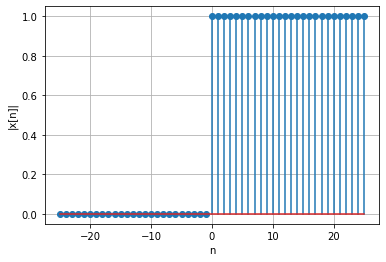
\includegraphics[width=\columnwidth]{1.png}
 \caption{$x_1(t)$ and $x_2(t)$}
 \end{figure}
 
  \begin{figure}[!htp]
\centering
 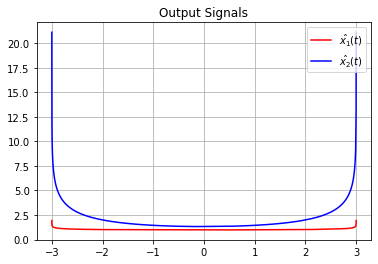
\includegraphics[width=\columnwidth]{2.png}
 \caption{$\hat{x_1}(t)$ and $\hat{x_2}(t)$}
 \label{fig2}
 \end{figure}
 
  \begin{figure}[!htp]
\centering
 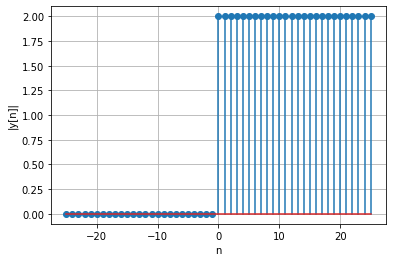
\includegraphics[width=\columnwidth]{3.png}
 \caption{Law of Additivity}
 \end{figure}
 
  \begin{figure}[!htp]
\centering
 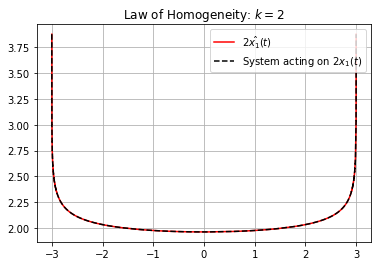
\includegraphics[width=\columnwidth]{4.png}
 \caption{Law of Homogeneity}
 \end{figure}


\item \textbf{\underline{Time invariance}}\\
From \eqref{T} , to check for time-invariance, we would introduce a delay of $t_0$ in the output and input signals.\\
Now, we consider an input signal with a delay of $t_0$, given by $x(t-t_0)$, and let the corresponding output signal be given by $\hat{x}(t-t_0)$, then:
\begin{align}
    \hat{x}(t-t_0) &=\brak{\frac{1}{\pi (t-t_0)}}\ast x(t-t_0)\label{01}
\end{align}

Now, Delay the input signal and apply the system, then 
We can write $\hat{x}_1(t)$,
\begin{align}
\hat{x}_1(t)
    &= \brak{\frac{1}{\pi (t-t_0)}}\ast x(t-t_0)\label{00}
\end{align}

Using \eqref{00} in \eqref{01},
\begin{align}
    \hat{x}(t-t_0) =\hat{x}_1(t) 
\end{align}

Thus, the system is \textbf{time-invariant}.\\
$\therefore$ The hilbert transformer is a \textbf{linear time invariant system(LTI)}.

 \begin{figure}[!htp]
\centering
 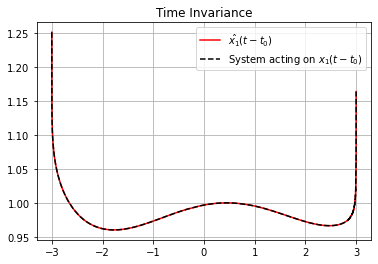
\includegraphics[width=\columnwidth]{5.png}
 \caption{Time Invariant}
 \end{figure}

\item {\textbf{\underline{Impulse response and non casual system}}}\\
Since the given system is an LTI system, it would possess an impulse response $h(t)$, which is the output of the system when the input signal is the Impulse function, given by $\delta(t)$. Thus,
\begin{align}
    h(t) = \frac{1}{\pi}\int\limits_{-\infty}^{\infty}\frac{\delta(k)}{t-k} dk\label{10}
\end{align}
The Impulse function can be loosely defined as:
\begin{align}
\nonumber    \delta(t) = 
    \begin{cases}
\infty & t = 0\\
0 & otherwise
\end{cases}
and \int_{-\infty}^\infty \delta(t)dt  = 1
\end{align}
\begin{align}
\int\limits_{-a}^{a} f(x)\delta(x-a) dx = f(a)\label{11}
\end{align}
By using \eqref{11} in \eqref{10},
\begin{align}
    h(t) = \frac{1}{\pi t}
    \label{H}
\end{align}
Here $h(t)$ is non zero for $t<0$.

Using \eqref{def}, That implies Hilbert transform is non casual system.
 \begin{figure}[!htp]
\centering
 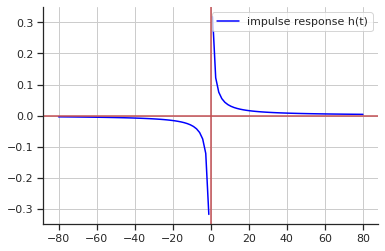
\includegraphics[width=\columnwidth]{hyp.png}
 \caption{Impulse response $h(t)$}
 \end{figure}
 
$\therefore$ Hilbert transformer is a non casual system.


\item {\textbf{\underline{Low-pass system}}}

Using \eqref{newdef} and by observing the Fig.\ref{figx3}, We can observe that the output signal consists of signal component corresponds to all frequencies i.e., there is no such cutoff frequency observed. 

  \begin{figure}[!htp]
\centering
 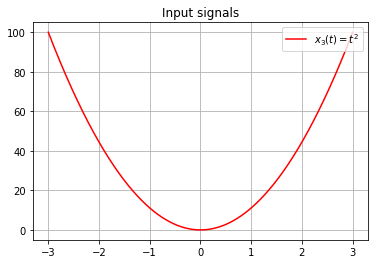
\includegraphics[width=\columnwidth]{x_31.png}
 \caption{Input signal $x_3(t)=t^2$}
 \end{figure}
 
  \begin{figure}[!htp]
\centering
 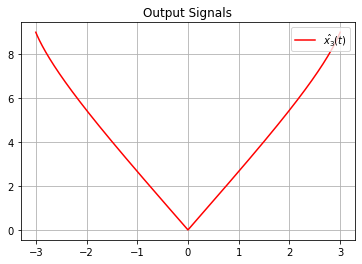
\includegraphics[width=\columnwidth]{x_32.png}
 \caption{Output signal $\hat{x_3}(t)$}
 \label{figx3}
 \end{figure}

\newpage
$\therefore$ We can say that the hilbert transform is \textbf{not a low-pass system}.
\end{enumerate}

$\therefore$ Correct option is \textbf{2) Non casual system}.
\end{proof}
\end{document}
